% !TEX encoding = UTF-8 Unicode

\documentclass[a4paper]{article}
\usepackage[utf8]{inputenc}
\usepackage{color}
\usepackage{url}
\usepackage[T2A]{fontenc} 
\usepackage[utf8]{inputenc} 
\usepackage{graphicx}
\usepackage[english,serbian]{babel}

\usepackage[unicode]{hyperref}
\hypersetup{colorlinks,citecolor=green,filecolor=green,linkcolor=blue,urlcolor=blue}


\begin{document}

\title{Skot Aronson \\
\small{Seminarski rad u okviru kursa\\Tehničko i naučno pisanje\\ Matematički fakultet}}

\author{Vidak Kozomara, Đorđe Milošević,\\Lazar Perišić, Aleksa Cvetković\\
vidak.kozomara@gmail.com, djordjem00@gmail.com,\\ lakiwow95@gmail.com, 013.aleksa@gmail.com, }

\date{oktobar 2019.}
\maketitle

\abstract{
  Ovaj rad predstavlja specifičnosti i zanimljivosti vezane za, kod nas, slabo poznatog
  naučnika, Skota Aronsona. Čovek, čiji je san kao jedanaestogodišnjaka bio da napravi svoju igricu \cite{thecomplexonaut}, danas je jedan
  od prestižnih naučnika u oblasti kvantnog i teorijskog računarstva.

\tableofcontents

\newpage

\section{Uvod}


\textbf{Skot Džoel Aronson} (eng. \textit{Scott Joel Aaronson}) je američki teorijski informatičar i profersor informatike na Univerzitetu u Ostinu, Teksas. Njegove primarne oblasti istraživanja su mogućnosti i limiti kvantnih računara kao i računarska teorija složenosti.

\vspace{5\baselineskip}



\begin{table}[h!]
\begin{center}


\begin{tabular}{|p{10.1cm}|} \hline


\begin{center}
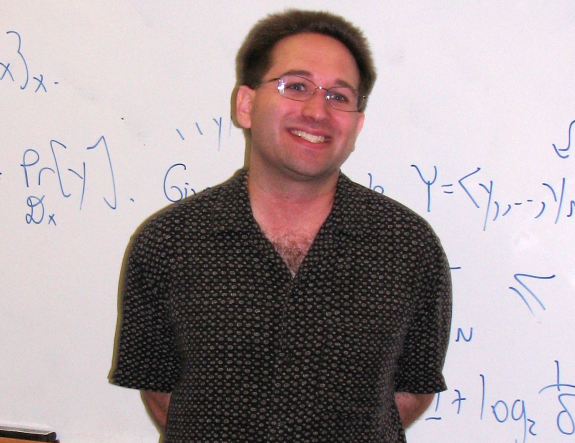
\includegraphics[scale=0.4]{Scott Aaronson.jpg}
\end{center}
\\ \hline

\end{tabular}

\hspace*{0.1cm}\begin{tabular}{|c|c|}
\textbf{Puno ime} & Skot Džoel Aronson\\ \hline
\textbf{Datum rođenja} & 21. maj 1981. \\ \hline
\textbf{Mesto rođenja} & Filadelfija, Pensilvanija\\ \hline
\textbf{Državljanstvo} & američko\\ \hline
\textbf{Zanimanje} & Teorijsko računarstvo i informatika\\ \hline
\textbf{Značajni radovi}  & "Ekvivalentnost uzorkovanja i pretraživanja"\\ \hline
\textbf{Supružnik} & Dana Moškovic\\ \hline
\textbf{Veb-sajt} & http://www.scottaaronson.com/blog/ \\ \hline

\end{tabular}


\end{center}
\end{table}

\newpage
\section{Mladost i obrazovanje}
Rođen je u Filadelfiji 21.maja 1981. godine. Odrastao je u Sjedinjenim Američkim Državama, 
ali je proveo jednu godinu u Aziji kada se njegov otac, naučni pisac, 
zbog promene posla preselio u Hongkong. \cite{thecomplexonaut} Pohađao je školu koja mu je omogućila da preskoči 
matematiku nekoliko godina, ali po povratku u SAD, obrazovanje mu je bilo ograničeno, dobijao je loše ocene i imao rasprave sa nastavnicima. 
\\[1\baselineskip]
Zatim se upisao u školu Klarkson, program za nadarene mlade osobe, vođen od strane Klarkson Univerziteta, koji je omogućio 
Aronsonu da se prijavi na koledže dok je bio tek prva godina srednje škole. Prihvaćen je na Kornel Univerzitet, gde je stekao zvanje diplomiranog inženjera iz informatike 2000. godine. 
Nakon toga, doktorske studije je završio u na Berkliju (Univerzitet Kalifornije) 2004. godine pod nadzorom Umeša Vaziranija.
\\[1\baselineskip]
Aronson je pokazao talenat za matematiku još u detinjstvu. Već u 11. godini je učio analizu, za koju su ga zainteresovali simboli iz dadiljine knjige. \cite{thecomplexonaut} 
Otkrio je programiranje u 11. godini, i osetio da njegovo znanje zaostaje za vršnjacima, koji su već programirali godinama. 
Prvi programski jezik koji je učio je bio Bejsik (engl. BASIC). Delimično zbog toga što je Aronson učio naprednu matematiku pre 
nego što je počeo da se bavi računarskim programiranjem, osetio je privlačnost teorijskog računanja, posebno računske složenosti. 
Sa 14 godina čita popularan artikal o kvantnim kompjuterima koji ga privlači toj oblasti. 
\\[1\baselineskip]
Kao tinejdžer, baš u vreme kada je učio o algoritmima vezanim za kvantne kompjutere, 
imao je letnju praksu u Bel laboratorijama. Ta praksa nije imala nikakve veze sa kvantnim kompjuterima međutim tamo je upoznao čoveka koji je izmislio Groverov algoritam, 
Lova Grovera, koji mu je ponudio praksu za sledeću godinu. \cite{praksa} Na Kornelu, zainteresovao se za kvantno programiranje, i posvetio se kvantnom programiranju i računskoj složenosti.
\section{Karijera}
Nakon postdoktorata na Institutu za napredne studije i Univerzitetu u Voterlu, 
uzeo je fakultetsku poziciju na MIT-u. Njegova primarna oblast je kvantno programiranje i računarska teorija složenosti. 
\\[1\baselineskip]
U leto 2016. godine napušta Masačusetski tehnološki institut (MIT) i odlazi na Univerzitet u Teksasu, 
u Ostinu, kao profesor veka u oblasti informatike i kao osnivač novog kvantnog informativnog centra.
\\[1\baselineskip]
Pored karijere u obrazovanju, Skot Aronson je radio i za neke kompanije poput:
\begin{itemize}
\item VMWare
\item Pivotal Software Inc
\item Greylock Partners
\item Cloudera Inc
\item Medallia Inc
\end{itemize}
Trenutno radi kao glavni direktor prihoda u kompaniji Cloudera. \cite{company}


\subsection{Nagrade}
\begin{itemize}
\item Jedan od dva dobitnika nagrade Alan T. Vaterman (eng. \textit{Alan T. Waterman}) za 2012. godinu \cite{nagrada1}
\item Nagrada za najbolji rad u računarstvu u Rusiji 2011. godine za rad \textit{"Ekvivalentnost uzrokovanja i pretraživanja"(engl. The Equivalence of Sampling and Searching)} 
\item 2017. Simons istražitelj \cite{nagrada2}
\end{itemize}


\section{Marketinški plagijat}
U Oktobru 2007. godine Skot Aronson je optužio marketinšku agenciju Lav Komunikejšns (eng. \textit{Love Communications}) 
za prisvajanje dela njegovog predavanja u jednoj marketinškoj kampanji za Riko (eng. \textit{Ricoh}). Nakon razgovora sa advokatom, 
bio je siguran da ima dobar slučaj, ali da nema ni novca ni vremena da se tuži. Zbog toga, predlaže nagodbu. 
Marketinška agencija prihvata nagodbu ali sa mnogo manjom odštetom od one koju je on predložio. 
Aronson je rekao da u tom trenutku nije imao energije da se cenka sa njima i prihvatio je 
nagodbu u iznosu od 5000 dolara koje će oni donirati nekim organizacijama koje popularizuju nauku u Australiji. 
Iako su prihvatili nagodbu, generalni direktor Lav Komunikejšnsa je izjavio da su verovatno trebali da ga pitaju 
pre nego što su iskoristili njegove reči ali da ne misle da su prekršili autorska prava. \cite{ad}

\section{Popularni radovi}
Skot Aronson je osnivač elektronske biblioteke algoritama i problema zvanom ``Complexity Zoo'' iz polja 
informatike koja čuva i sortira probleme po klasi kompleksnosti. On je takođe osnivač bloga ``Shtetl-Optimized'' \cite{shtetloptimized} kao i eseja ``Who Can Name The Bigger Number?'' \cite{whocannamethebiggernumber}. 
\\[1\baselineskip]
On je držao predavanje o kvantnoj izračunljivosti, sa kog su beleške dostupne na internetu. 
Napisao je knjigu koja je objavljena od strane Novina Kembridž Univerziteta \cite{knjiga}. 
Koncepti koje pokriva knjiga su kasnije sažeto objašnjeni u članku ``Why Philosophers Should Care About Computational Complexity''. 
Od tada je objavio još jednu knjigu nazvanu po malopre pomenutom predavanju koja se zasniva na konceptima sa predavanja.



\section{Zaključak}
Kroz ovaj rad možete se upoznati sa činjenicama i zanimljivostima vezanim za Skota Aronsona. Iako mlad, već je osvojio neke prestižne nagrade i postao cenjen u naučnom svetu.





\addcontentsline{toc}{section}{Literatura}
\appendix
\bibliography{seminarski} 
\bibliographystyle{unsrt}


\appendix


\end{document}
